\section{Evaluation}

Over 12 months, several studies were conducted to answer new research questions or rephrase existing ones. These studies are grouped in 3 phases, each tested a different version of \chameleon{} with human participants. The number of participants and their haskell experience is shown in the table below. 



A summary of the timeline of the user studies, their major questions and conclusions is given in Figure~\ref{fig:timeline}.

\begin{figure}[h]
    \centering
    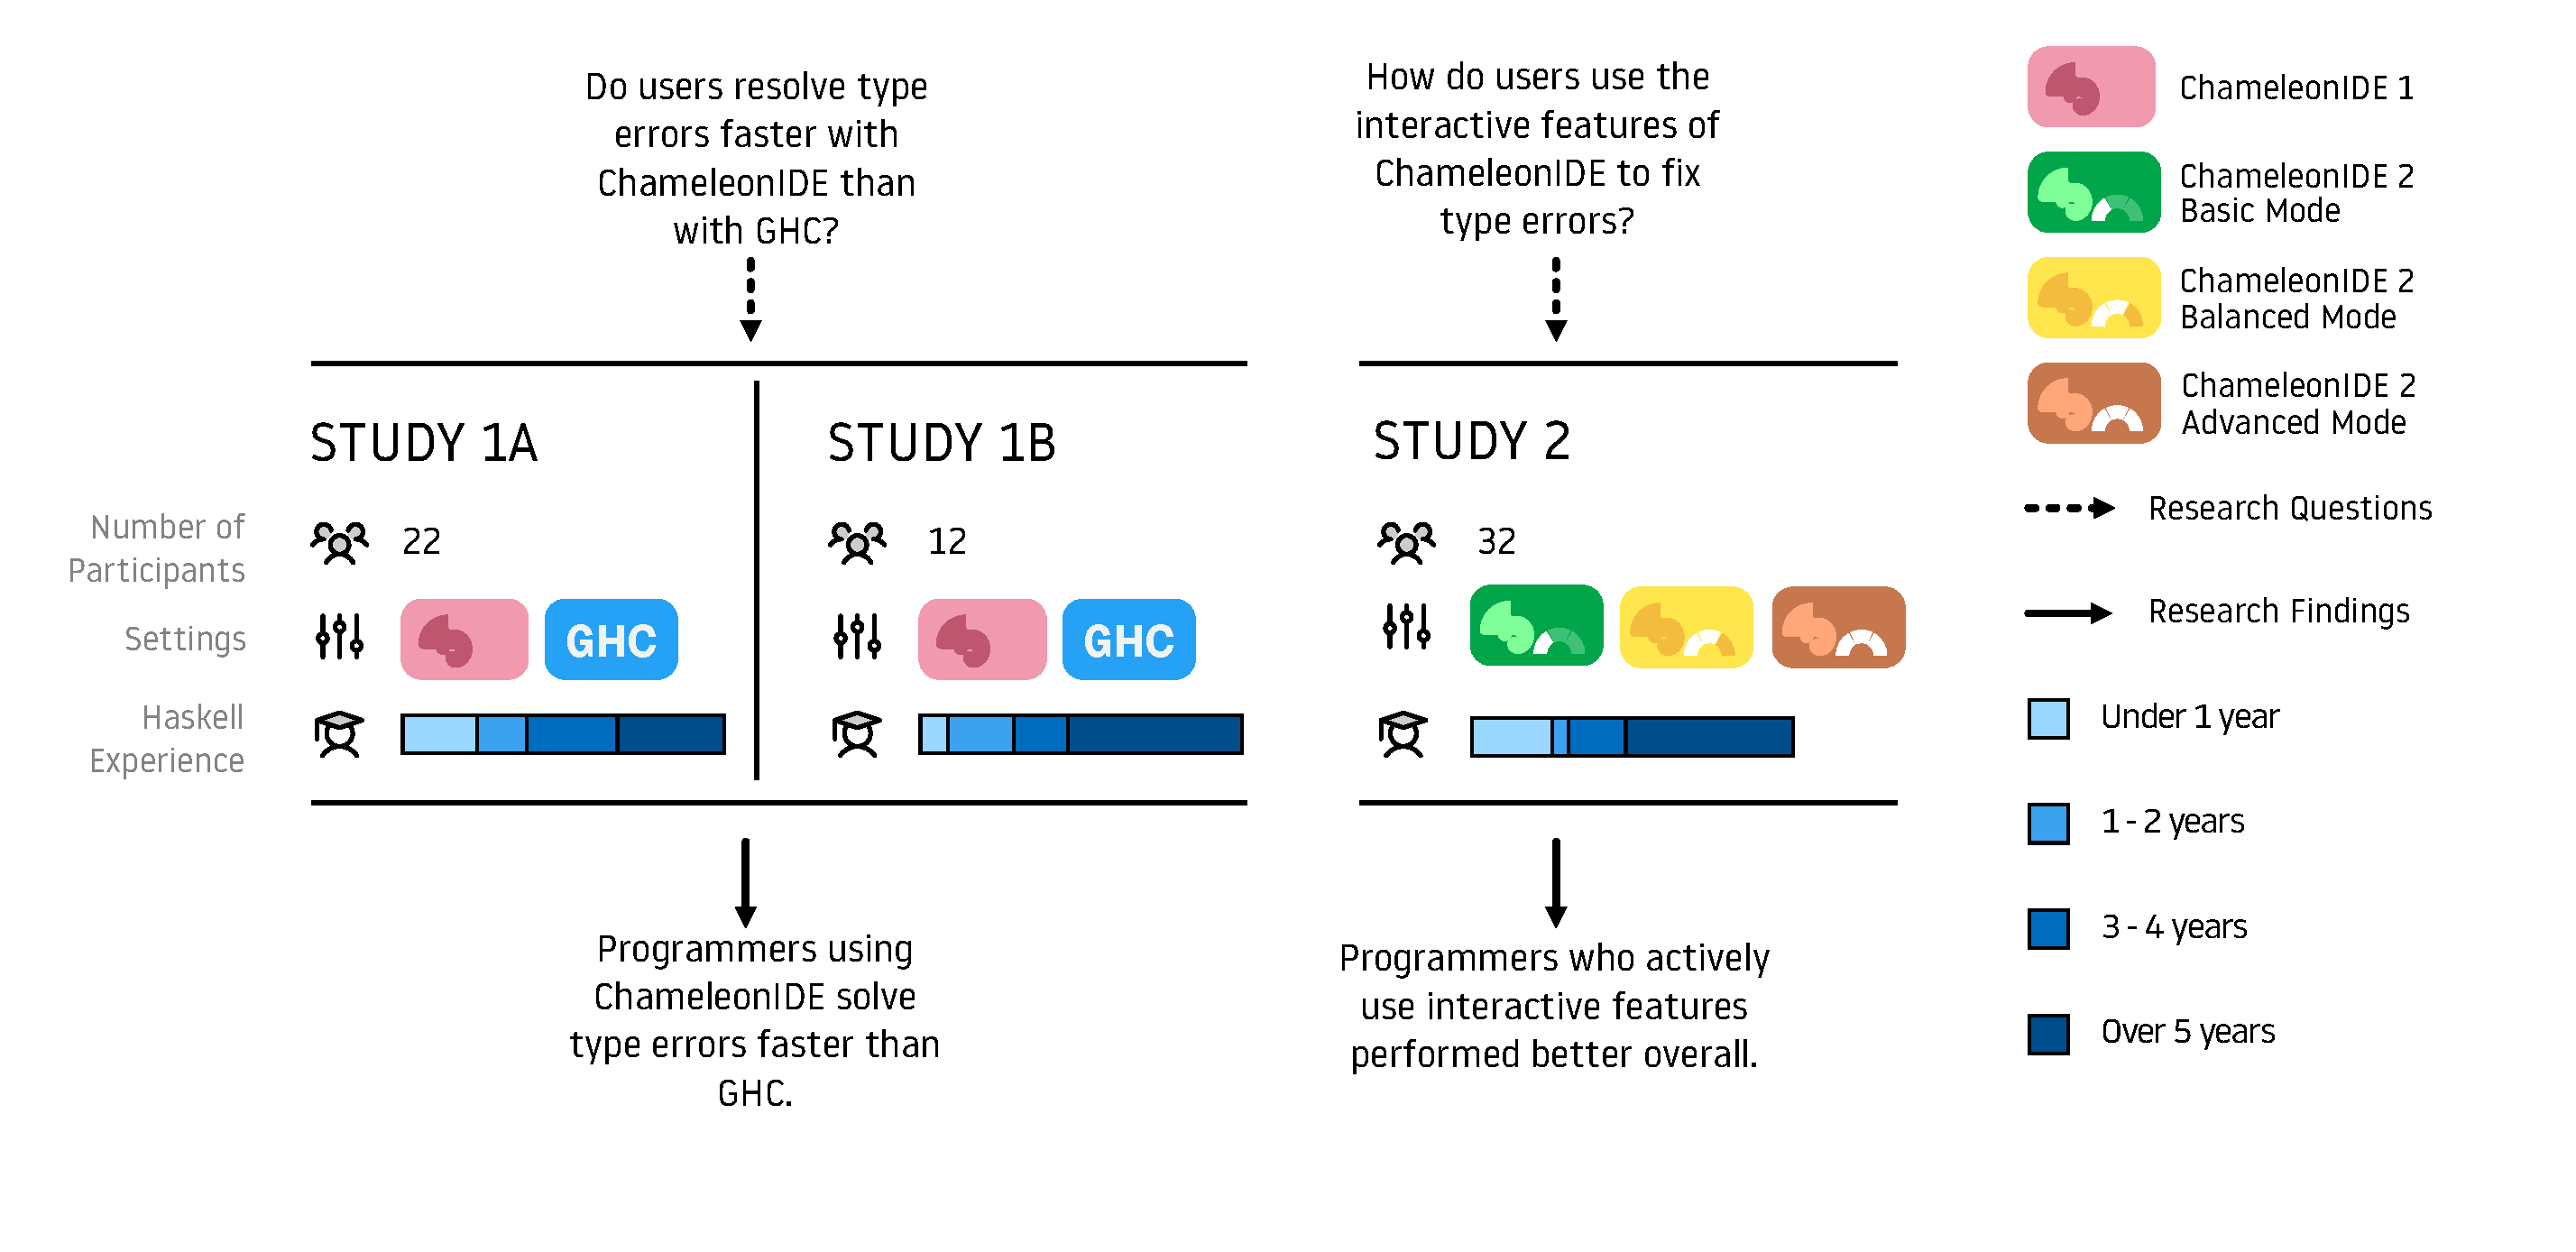
\includegraphics[width=\linewidth]{images/timeline.pdf}
    \caption{The timeline of \chameleon{}  development and 
    evaluation.}
    \label{fig:timeline}
\end{figure}

\subsection{Experiment Design}
\subsubsection*{\textbf{Recruitment}}

Participant recruiting channel was the social news aggregation website Reddit. Specifically, our user study advertisements were posted in the Haskell programming language community "r/haskell" and a general programming language-focused community "r/programminglanguages". Recruiting from social media allowed us to access a more diverse demographic that better represent the true population of Haskell programmers. The participation is fully anonymized. The detailed ethical implications of these experiments are reviewed and approved by the IRB of the institution of the authors.

One consequence of our recruiting approach is it is harder for previous participants to enter an later study. To minimise the lurking variable of previous experience, we use new code challenge every study and conduct trial runs in every study to bring new participants up to speed.

\subsubsection*{\textbf{Experiment setting}}
The experiment took place remotely and unsupervised. Participants took the study online via web browser and at the physical venue of their choosing. All user studies use a web-based debugging environment developed by the authors. Conducting the studies online helped us avoid variation when performing tasks in unfamiliar places and using different setups. The downside is that to intervene when a user encounters bugs or usability issues mid-study is impossible. To ensure there is no major usability issue that could lower the quality of data collection, we conducted cognitive walkthroughs and sandbox pilots before running each study.



\subsubsection*{\textbf{Training and group assignment}}
After consent, participants received interactive training on every function of the tool interface and interactive features. Participants were also shown the important functionalities of the tool interface in a summarized cheat sheet. Participants had access to the cheat sheet at all times during the study. Participants were given 4 trial runs (2 for each setting) before the data collection starts. 

All the user studies used a within-subject design to evaluate the effectiveness of different tools or feature sets while counterbalancing the difference in programming proficiency between participants. In each user study, participants were required to complete a series of programming tasks (8 for user studies 1 - 3, 9 for user study 4). At each task, a participant receives a single Haskell file that contains one or more type errors. The participant was asked to make the code type check with the help of the tool given for this task.


% During each study, a participant received two (user studies 1 - 3) or three (user study 4) different debugging tools. The debugging tools were different systems (user studies 1 - 3) or different feature sets of the same system (user study 4). For each participant, the debugging tools alternative through consecutive tasks to ensure the fatigue level does not impair the rigorousness of data collection.

\subsubsection*{\textbf{Measurement}}
Time is measured from the start of each task to the first time the program is successfully type-checked and also passes all the functional tests. The data is automatically recorded by the online debugging environment. To not introduce a barrier to completing the study, every task can be skipped if the participant made three attempts or spent over 1 minute on the task.


After completing all the tasks (8 in user studies 1-3, 9 in user study 4), users are prompted to fill in a debriefing survey. The survey questions include their Haskell programming experience and feedback on the tools and feature sets participants used during the study.


We used an browser session recording tool~\cite{openreplay} to record the user study sessions. These recordings are used to find usability issues in the study and recognize general patterns. However, the recording technology does not provide high enough sampling rate for us to be confidently used for rigorous analysis.

\subsection{\chameleon{} User Studies}


\subsubsection{\textbf{Version 1}}  
\chameleon{} version 1 provides the rewrite of the Chameleon type inference engine and the type compare tool to show the alternative types and possible error locations in matching colors.

\begin{figure}[h]
    \centering
    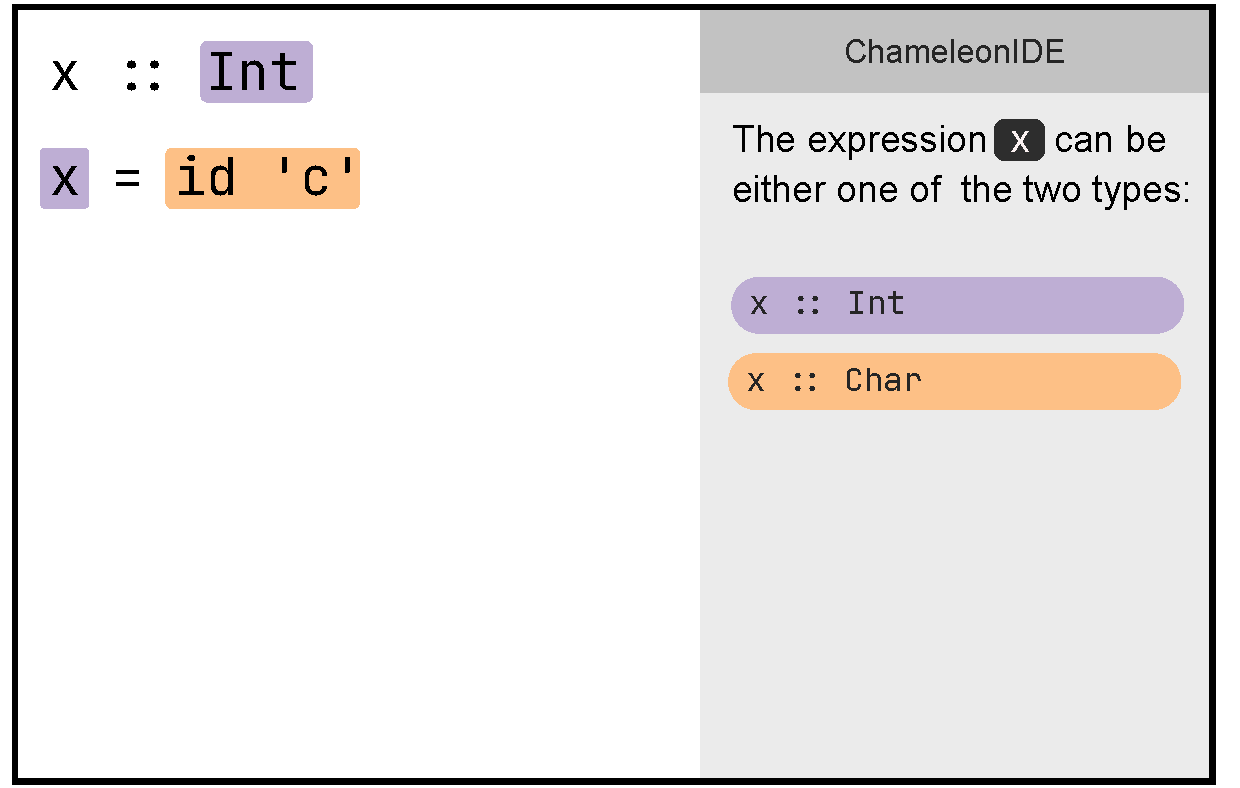
\includegraphics[width=\linewidth]{images/chameleon-v1.pdf}
    \caption{
        \chameleon{} Version 1
        }
    \label{fig:chameleon-v1}
\end{figure}

Two user studies were conducted to test \chameleon{} version 1, to compare the effectiveness of solving type errors using \chameleon{} and GHC compiler error messages. We choose GHC compiler error messages as the baseline because it is the canonical tool for working with type error in Haskell. Although high-level tools like Haskell Language Server exist, they generally relay the GHC error messages verbatim. 


Eight tasks were given in both studies. In the first study, the tasks were taken from a exercises from the exercises of the Haskell programming units. These tasks cover a variety of type errors. \tf{break down the type error classes.} However these tasks, as shown from the result and feedback of user study 1, were too simple to fully evaluate the two options. In the second study, the tasks are sourced from the top 20 Haskell topics on GitHub~\cite{githubHaskell}. The authors manually added type errors. 

\begin{figure}[h]
    \centering
    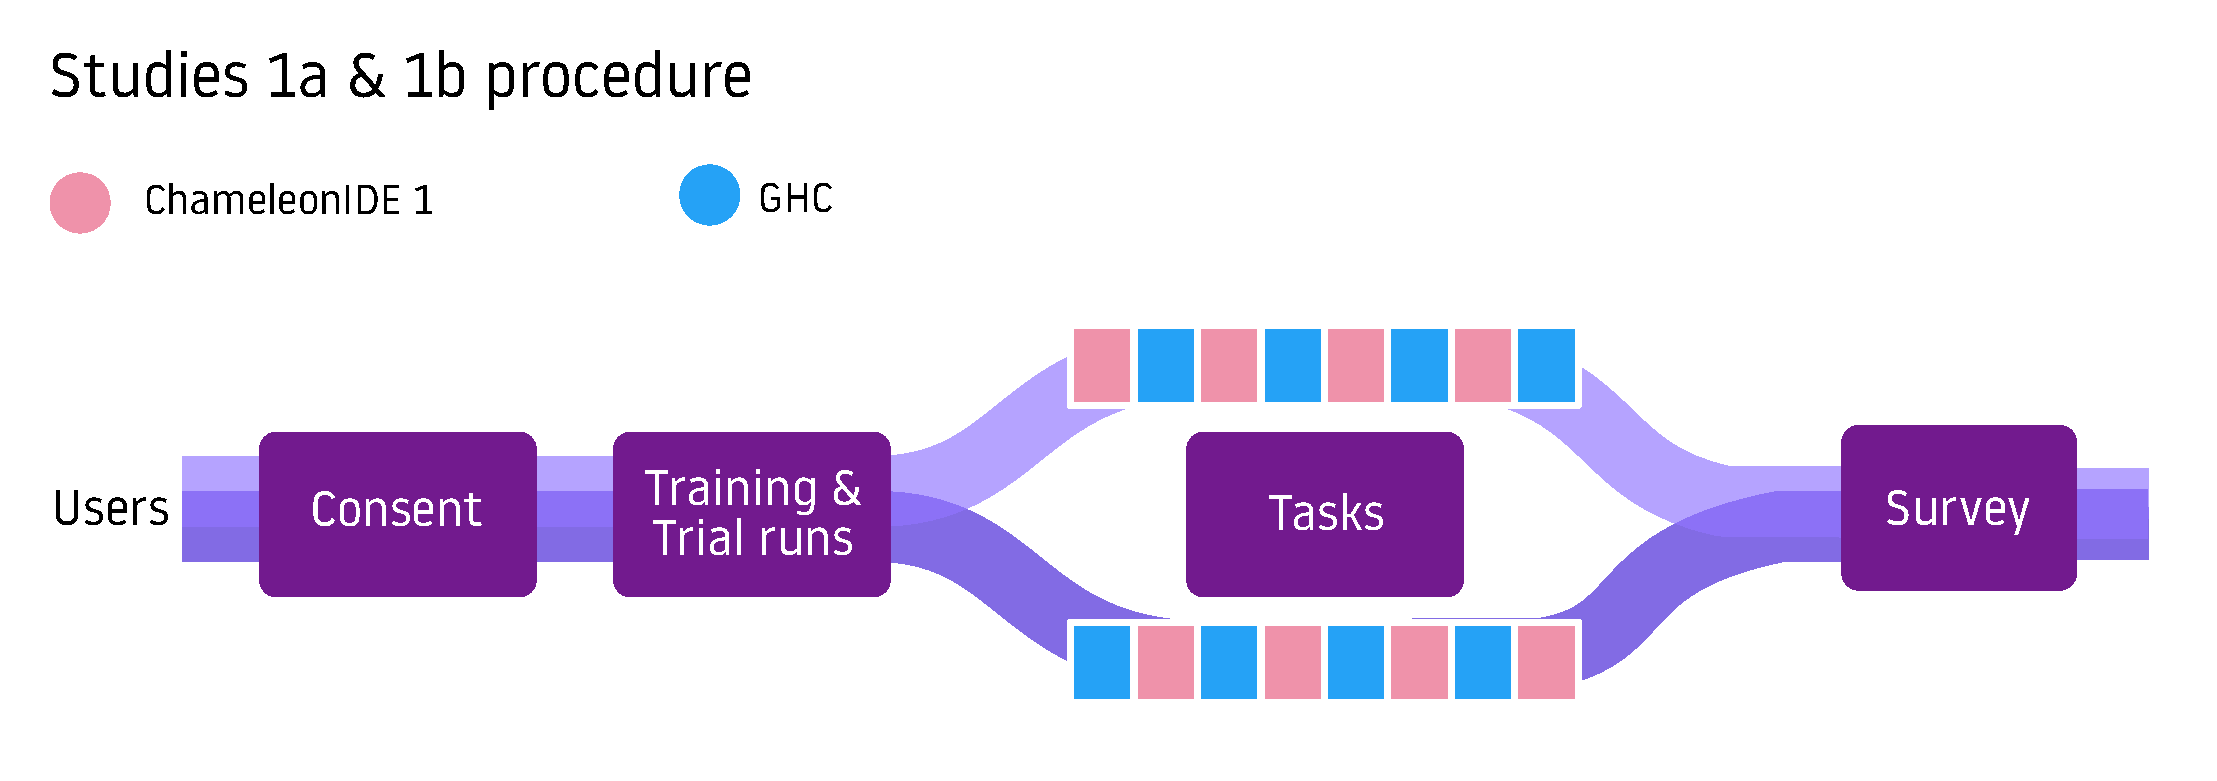
\includegraphics[width=\linewidth]{images/procedure-1.pdf}
    \caption{}
    \label{fig:study-process}
\end{figure}

% The study investigates the effectiveness of \chameleon{} compared to the GHC compiler error messages. We chose GHC compiler error messages as it is the canonical tool for debugging type errors in Haskell. Although high-level tools like Haskell Language Server exist, they relay the GHC error message verbatim for type errors. Participants are asked to complete 8 tasks. The tool participants used during each task alternated between \chameleon{} and GHC. Task programs were sourced from HaskellWiki \cite{haskellwiki}. The author manually added type errors. The errors cover a range of common Haskell type errors, including abstract data types, wrong arity, control expressions (if and case), infinite types, and tuples. The lines of code (LoC) range from 7 to 17 (mean = 11, median=10.5).


% In total 39 participants finished the study. Among them, 12 participants have over five years of Haskell experience, and 5 participants have three or four years of Haskell experience. And 8 participants have one or two years of experience, and 5 participants used Haskell for under a year. The rest left the question unanswered.

\begin{figure}[h]
    \centering
    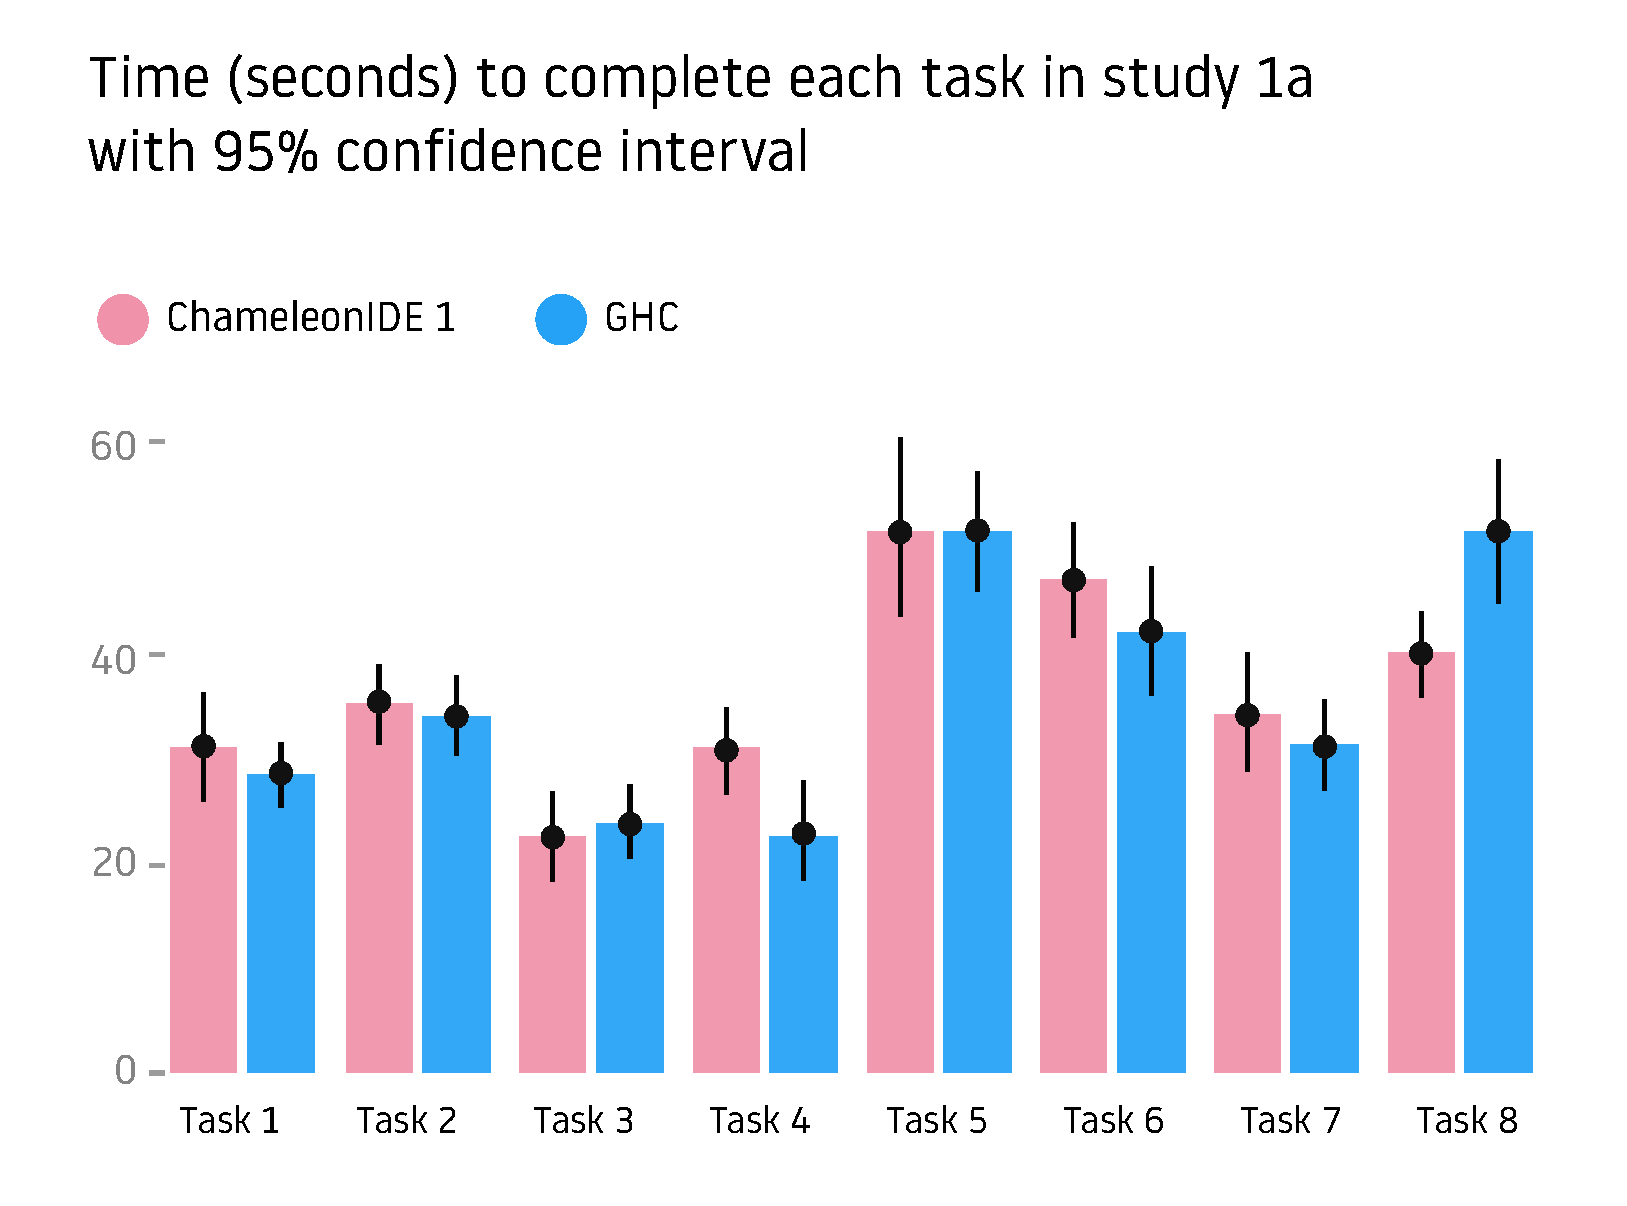
\includegraphics[width=\linewidth]{images/user-study-1a.pdf}
    \caption{Time to complete by task in user study 1a with confidence interval}
    \label{fig:r1-analysis}
\end{figure}


\begin{figure}[h]
    \centering
    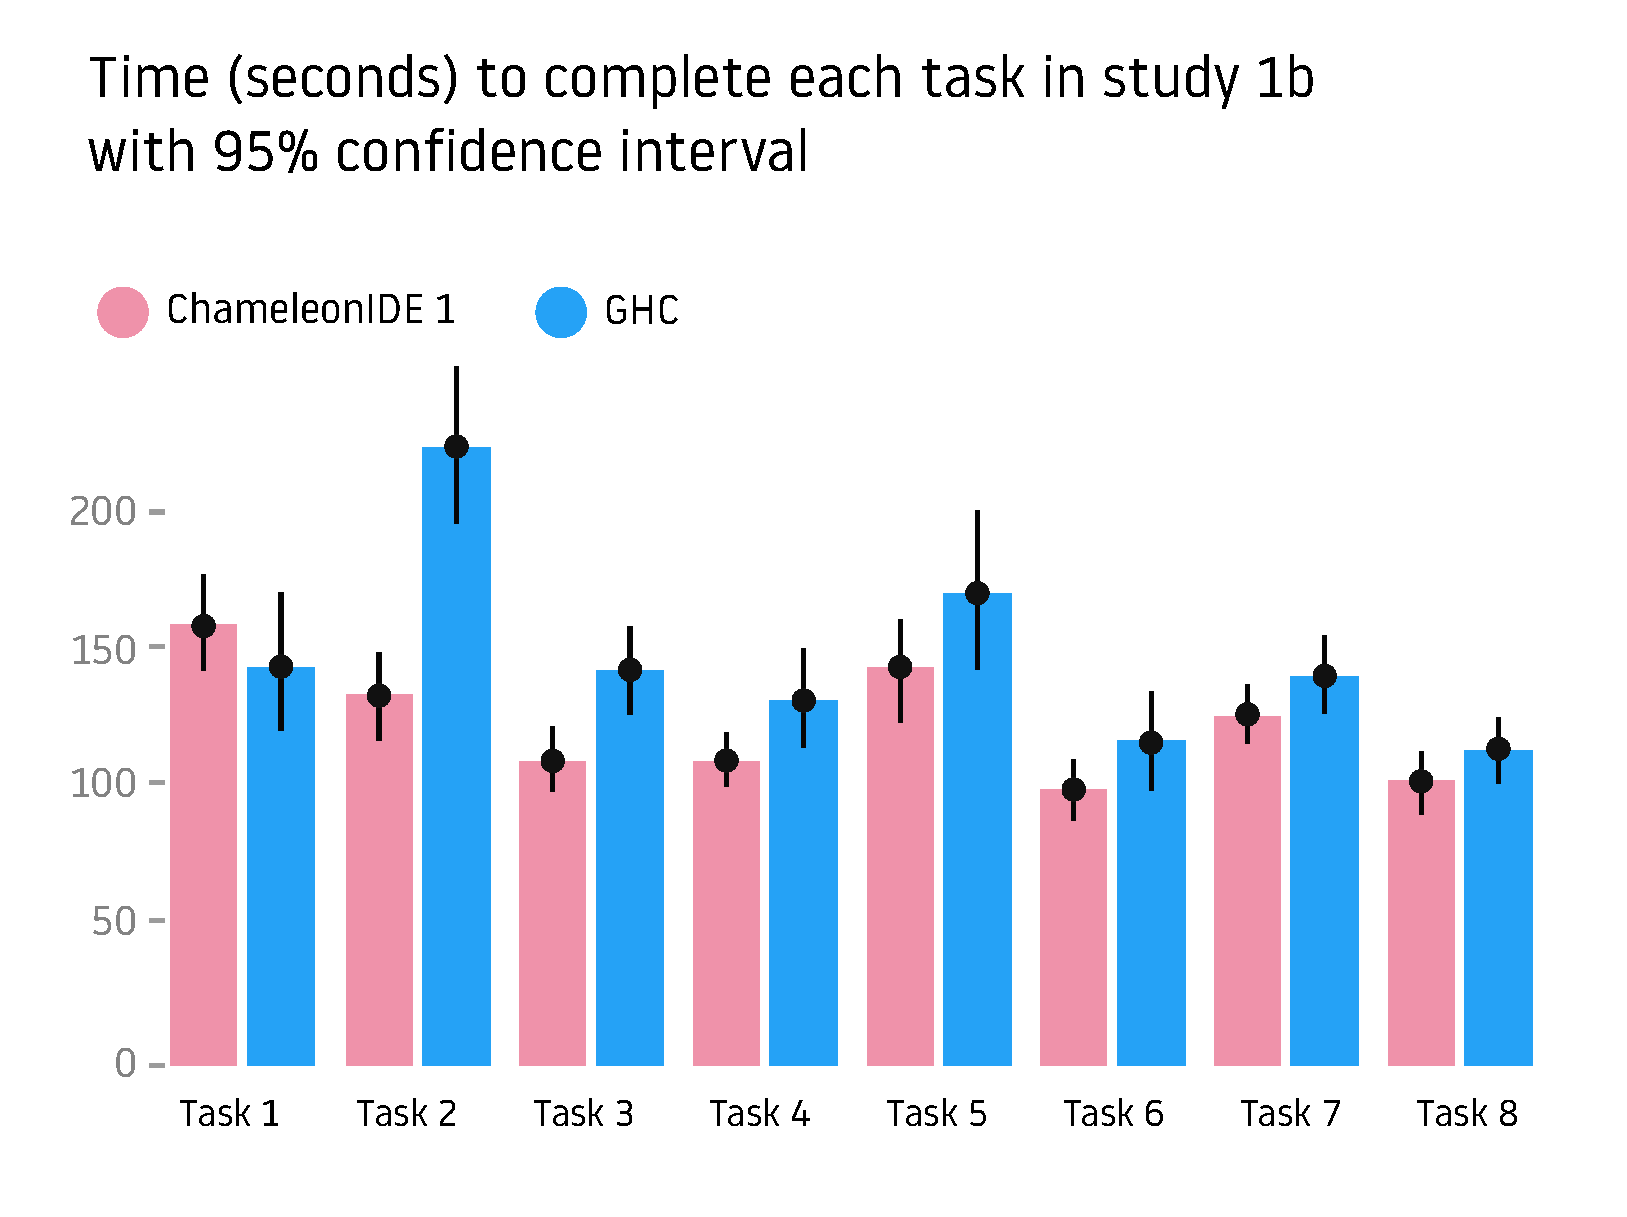
\includegraphics[width=\linewidth]{images/user-study-1b.pdf}
    \caption{Time to complete by task in user study 1b confidence interval}
    \label{fig:r2-analysis}
\end{figure}

\subsubsection*{\textbf {Results}}

From the data collected during user study 1 (\ref{fig:r1-analysis}), we could not identify which group performed better (p-value =0.2041, Wilcoxin signed test). For the trivial challenges we set for users, the individual differences are generally more significant than differences between treatments. 
The most common feedback (7 out of 35) from the user study 1 was that the tasks were too trivial to invite meaningful evaluation. One participant put it, "Looks nicer than GHC, but without trying it on something more complicated, I cannot conclude whether it would help me in practice".

One interesting exception is task 8, where the \chameleon{} group outperformed the GHC group more consistently and with a larger effect size (p-value = 0.002456, Wilcoxin signed test). The discrepancy is thought to be related to the nature of Task 8:
\begin{itemize}
    \item {It has a longer source file than other tasks (only shorter than task 6, but task
    6 contains two independent type errors while task 8 is one connected task
    error);}
    \item {It is more complex than others (involves abstract data types and function application); and
    }
    \item {
        GHC struggles to produce a relevant error message for this type of error.
    }
  \end{itemize}
It can be further shown by examining the process some participants took to solve the problem.

  

% \begin{figure}[H]
%     \centering
%     \Description{A screenshot from user study 1}
%     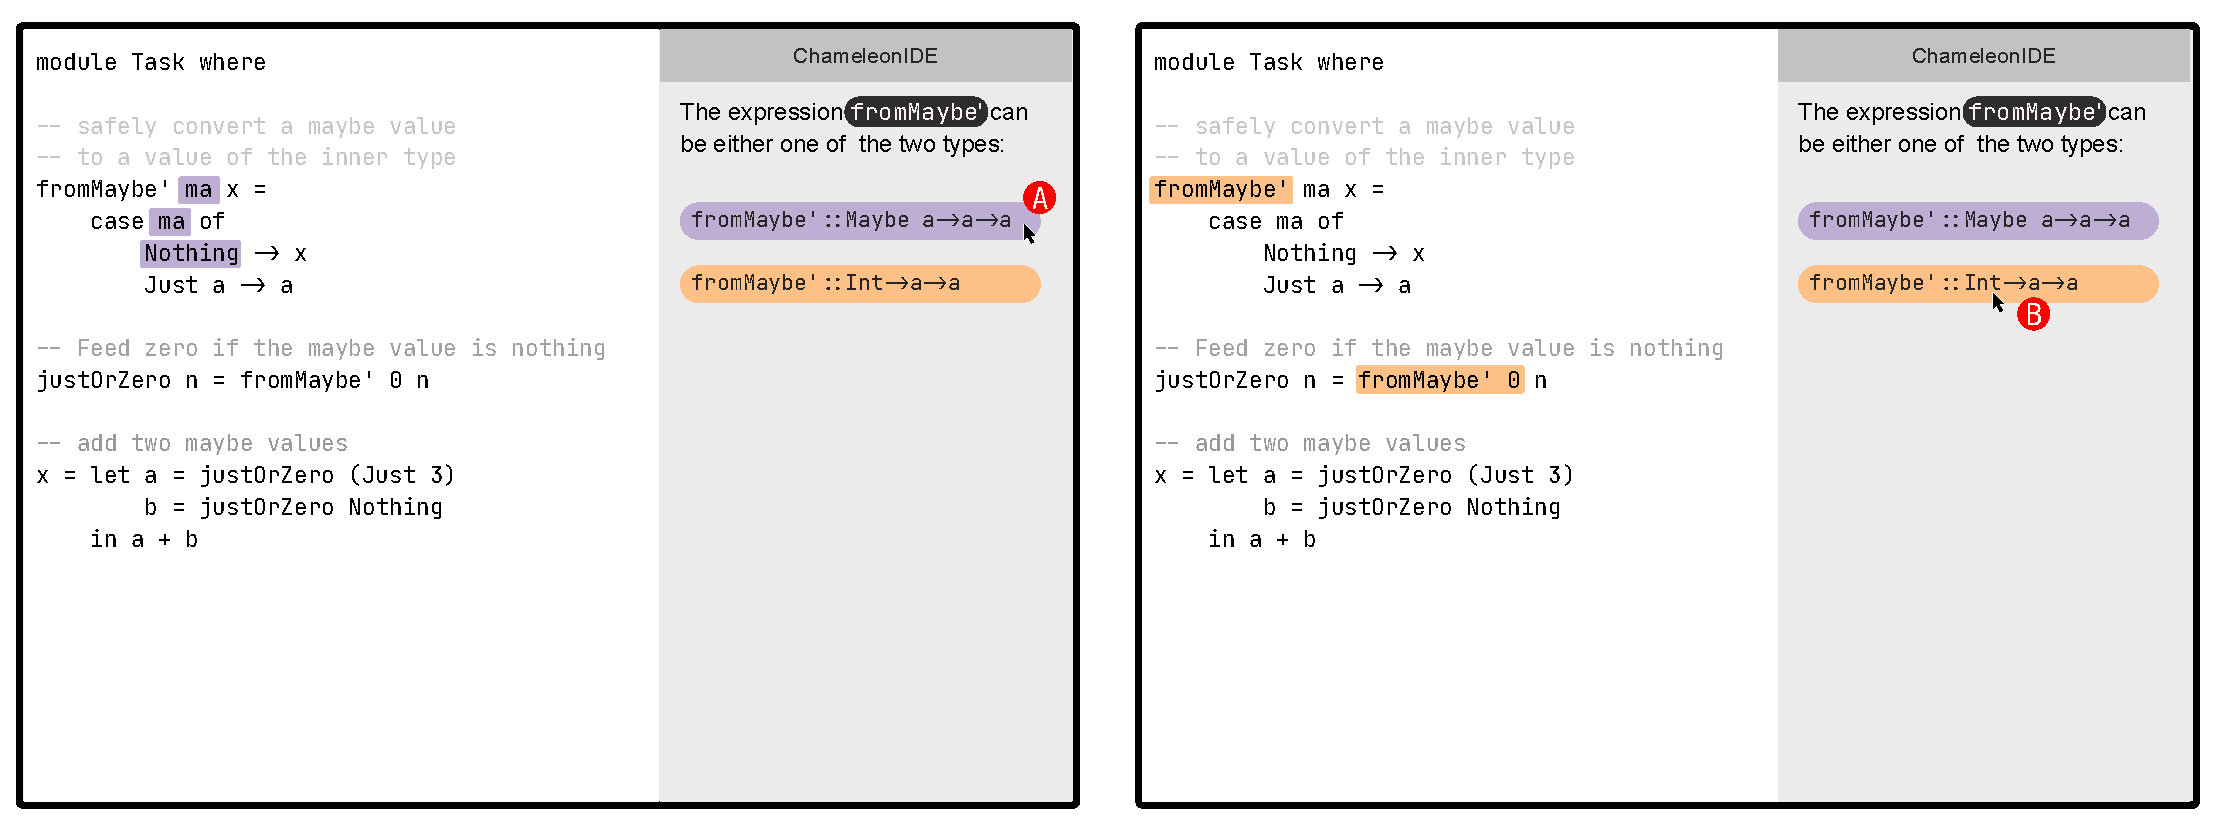
\includegraphics[width=\textwidth]{round1-screenshot.pdf}
%     \caption{
% One participant working with \chameleon{}  managed to identify the most probable location of the error (the application of `fromMaybe'` on line 11) by hovering over the two alternative types. The participant then quickly realized that the first argument `0` (highlighted in orange) is inconsistent with the definition where it is case matched to a `Nothing` value (highlighted in purple). After two retries with short hesitation the participant found the correct fix (by reversing the order of `0` and `n`).
%     }
%     \label{fig:r1-task8}
% \end{figure}


% \begin{figure}[htb]
%     \centering
%     \Description{A screenshot from user study 1}
%     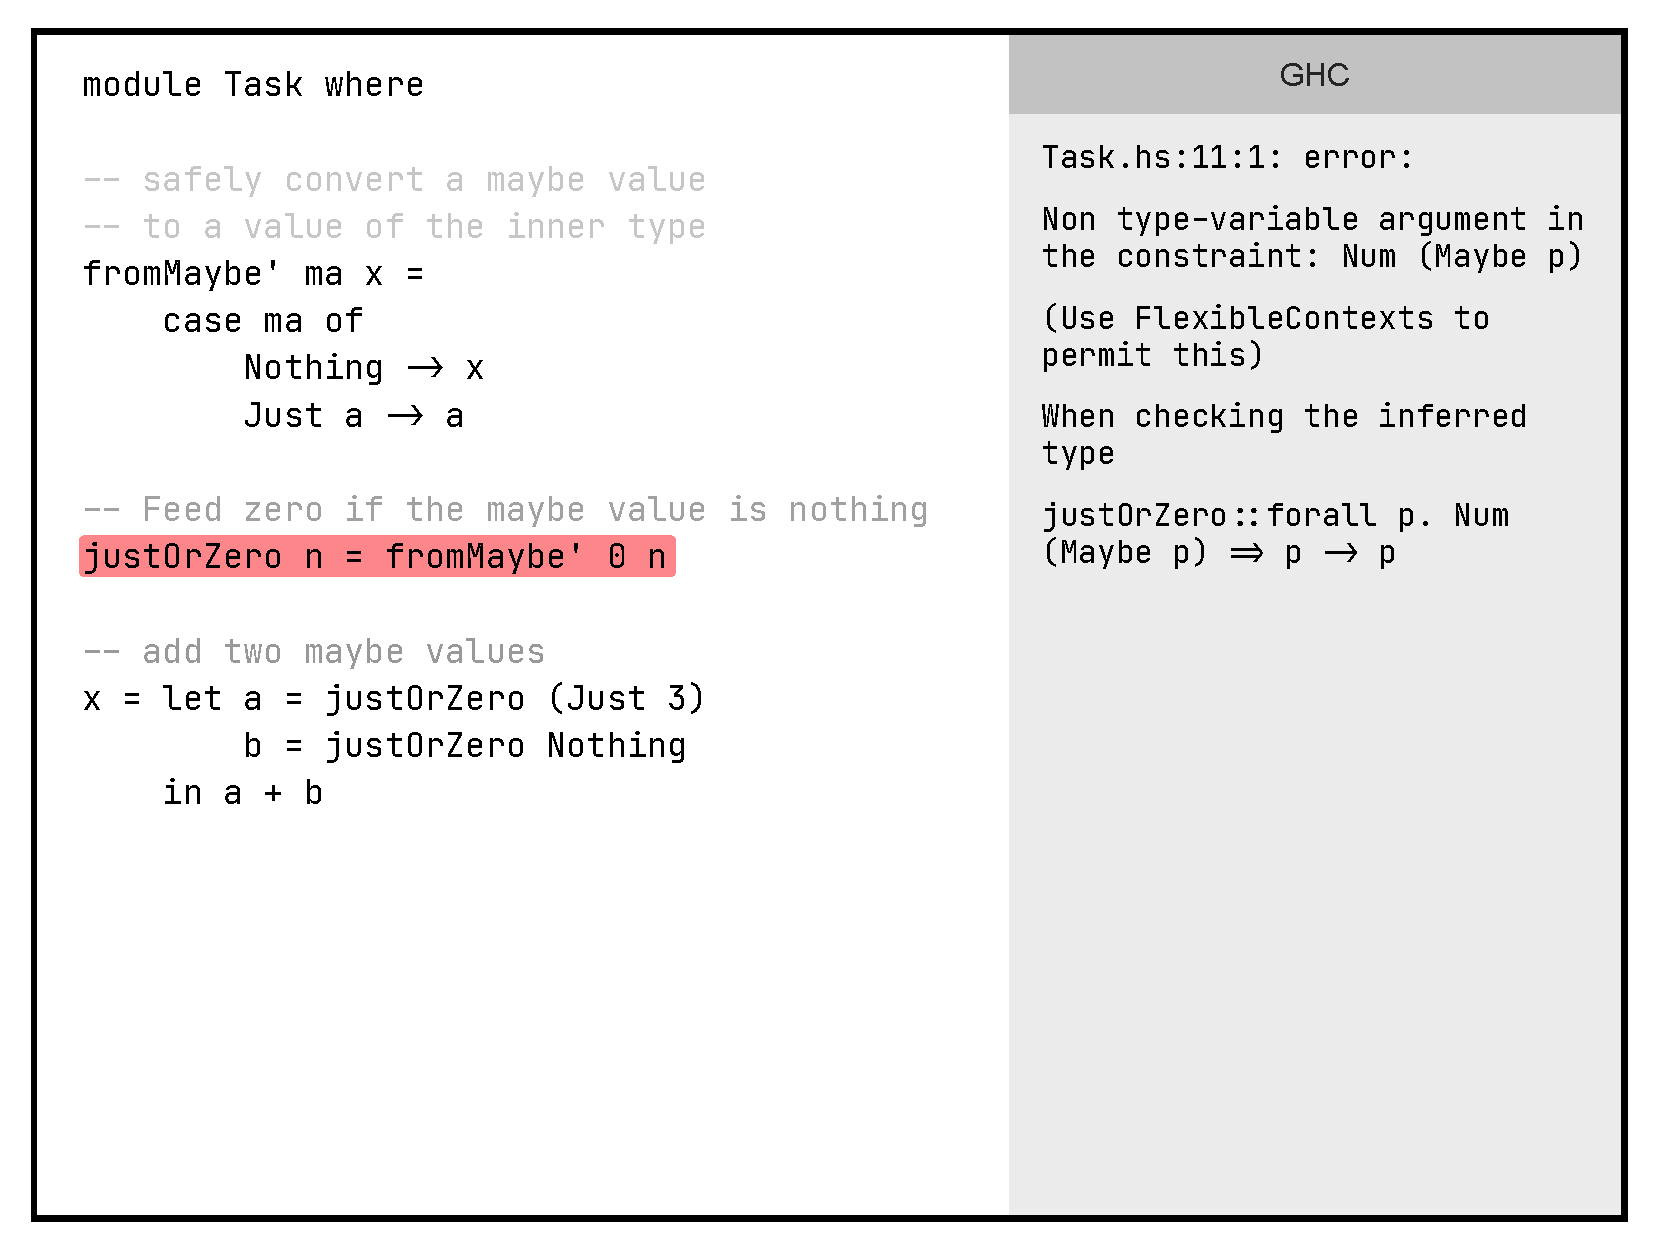
\includegraphics[width=\textwidth]{round1-screenshot-ghc.pdf}
%     \caption{
%         In task 8, participants using GHC took longer pauses at this task before committing to further investigation, either carefully reading the whole text or figuring out the meaning of the error message. The GHC error message is unfortunately unhelpful for this task.
%     }
%     \label{fig:task8-ghc}
% \end{figure}

In comparison, the \chameleon{} group solved the type error faster than the GHC group in almost all tasks (p =0.00742, Wilcoxin signed test) in study 2 (figure \ref{fig:r2-analysis}), barring task 1. The authors are unclear about the cause of low performance from \chameleon{} in task 1. It is suspected that some participants spent more time exploring the interface of \chameleon{} due to its unfamiliarity. From the video recordings, we saw many \chameleon{} users confidently skip reading unrelated chunks of code, while GHC users generally read through the whole program.


In harder problems and messier code, we notice programmers start to report the benefits of \chameleon{}. "Its most useful feature that I noticed was that it points out the locations of both conflicting uses; GHC often makes it difficult to figure out how it's coming to a conclusion about a type." reported one participant. "I think \chameleon{}  does a much better job than GHC's error messages. I like that it shows the sources for the type judgements. This makes it quite easy to figure out how to rectify errors." reported another participant.



\subsubsection{\textbf{Version 2}}  \label{sub:us4}

Version 2 is latest version of \chameleon{}. Not only the added features the deduction steps and candidate expressions are We designed an exploratory study to get better understanding of how users learn and use the multi-mode design of \chameleon{} version 3. During the study the initial mode of each task alternative through the three different modes, and repeat three cycles in nine tasks. The order of the three modes in each cycle is counterbalanced among all participants. However, participants are free to switch to other modes at any time. 


\begin{figure}[h]
    \centering
    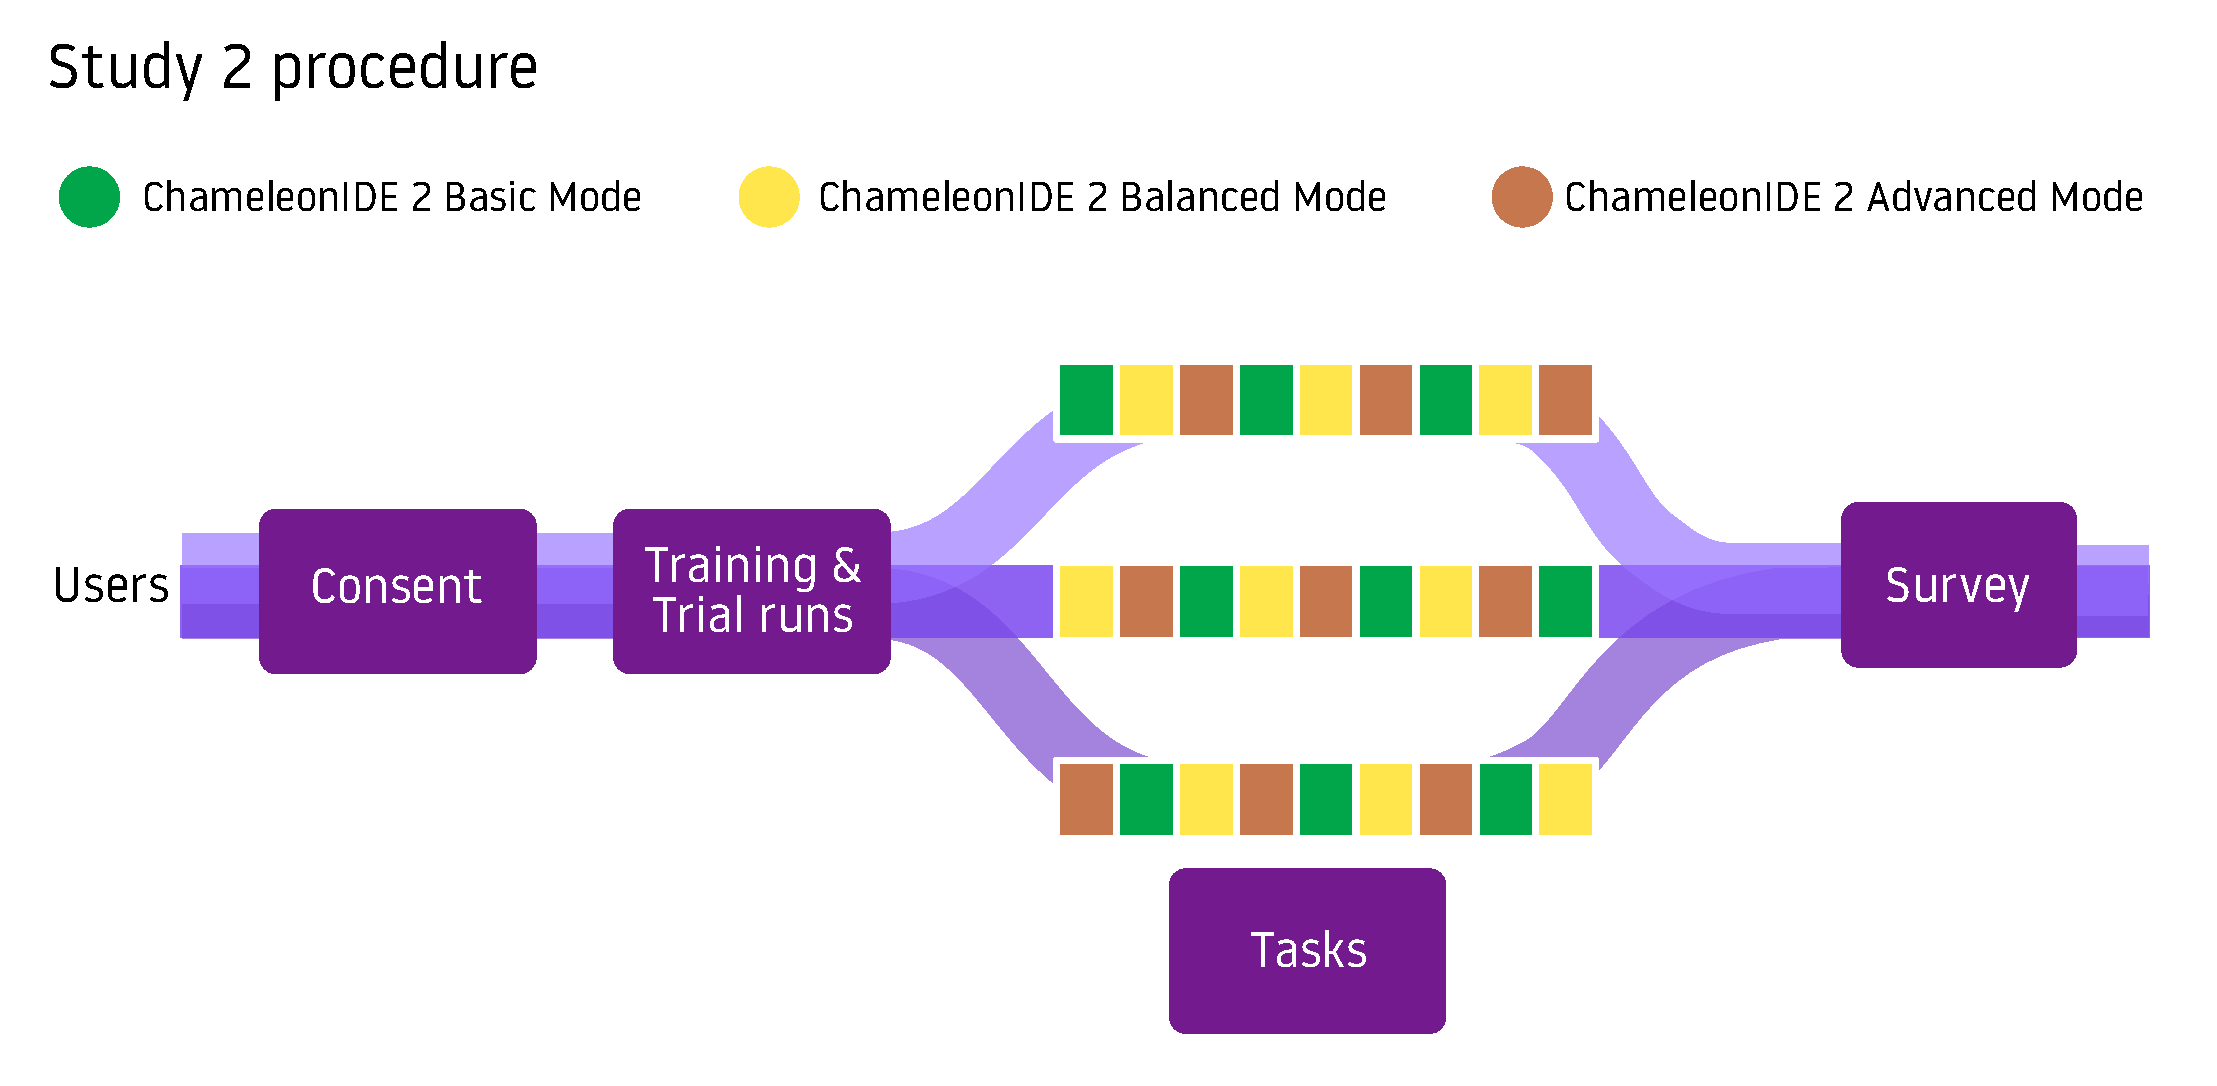
\includegraphics[width=\linewidth]{images/procedure-2.pdf}
    \caption{}
    \label{fig:study-process}
\end{figure}

\subsubsection*{\textbf{Results}} 

The study of \chameleon{} 2 is exploratory, in that we were hoping to let programmers discover their own way of using the tool. In post-hoc analysis of the collected log data, we were able to extrapolate some interesting patterns of how the tool was used. We share a few of our observations in this section.


The most striking feature of the data is users' tendency of using tools differ wildly. That is to say, some users used the feature extensively however some users completed the tasks without actively explore the given information. Based on this difference we divided the users into three groups.

\begin{tabularx}{\linewidth}{ 
  | >{\raggedright\arraybackslash}X 
  | >{\raggedright\arraybackslash}X  | }

    \hline
        Interaction level & Description \\ \hline
        Minimal Interaction & Users completed the tasks by making changes in source code, type checking, and reading error messages. \\ \hline
        Low Interaction & Users only actively used universal features in all modes, for example, hovering on "Possible type 1" and "Possible type 2" to narrow down error space. \\ \hline
        High Interaction & Users did everything from the Common feature group but used features specific to Balanced and Advanced mode, such as activating steps and expression cards. \\ \hline

\end{tabularx}



As shown in  figure \ref{fig:r4-analysis}, the time to complete each task roughly relates to the interaction level of participants. Participants with higher interaction levels generally performed better in the tasks, and the lowest level was worse (one-way ANOVA since we have three samples, p = 0.0368). The results from three tasks stand out from the general trend: in Tasks 4 and 6, higher interaction users performed worse, and in task 9, the general trend is exaggerated. As discussed in user studies 1 and 2, it is likely related to the nature of these tasks. Tasks 4 and 6 are shorter tasks in the study. The ideal fixes for these two tasks are placed relatively early in the source code (both in the first two lines of the source code). These may be useful because following the natural reading order will allow participants to skip lines on the bottom, and thus the advantage of \chameleon{} is less important. On the other hand, task 9 is the longest task of all. It also involves harder problems such as mutually recursive type definitions.

\begin{figure}[h]
    \centering
    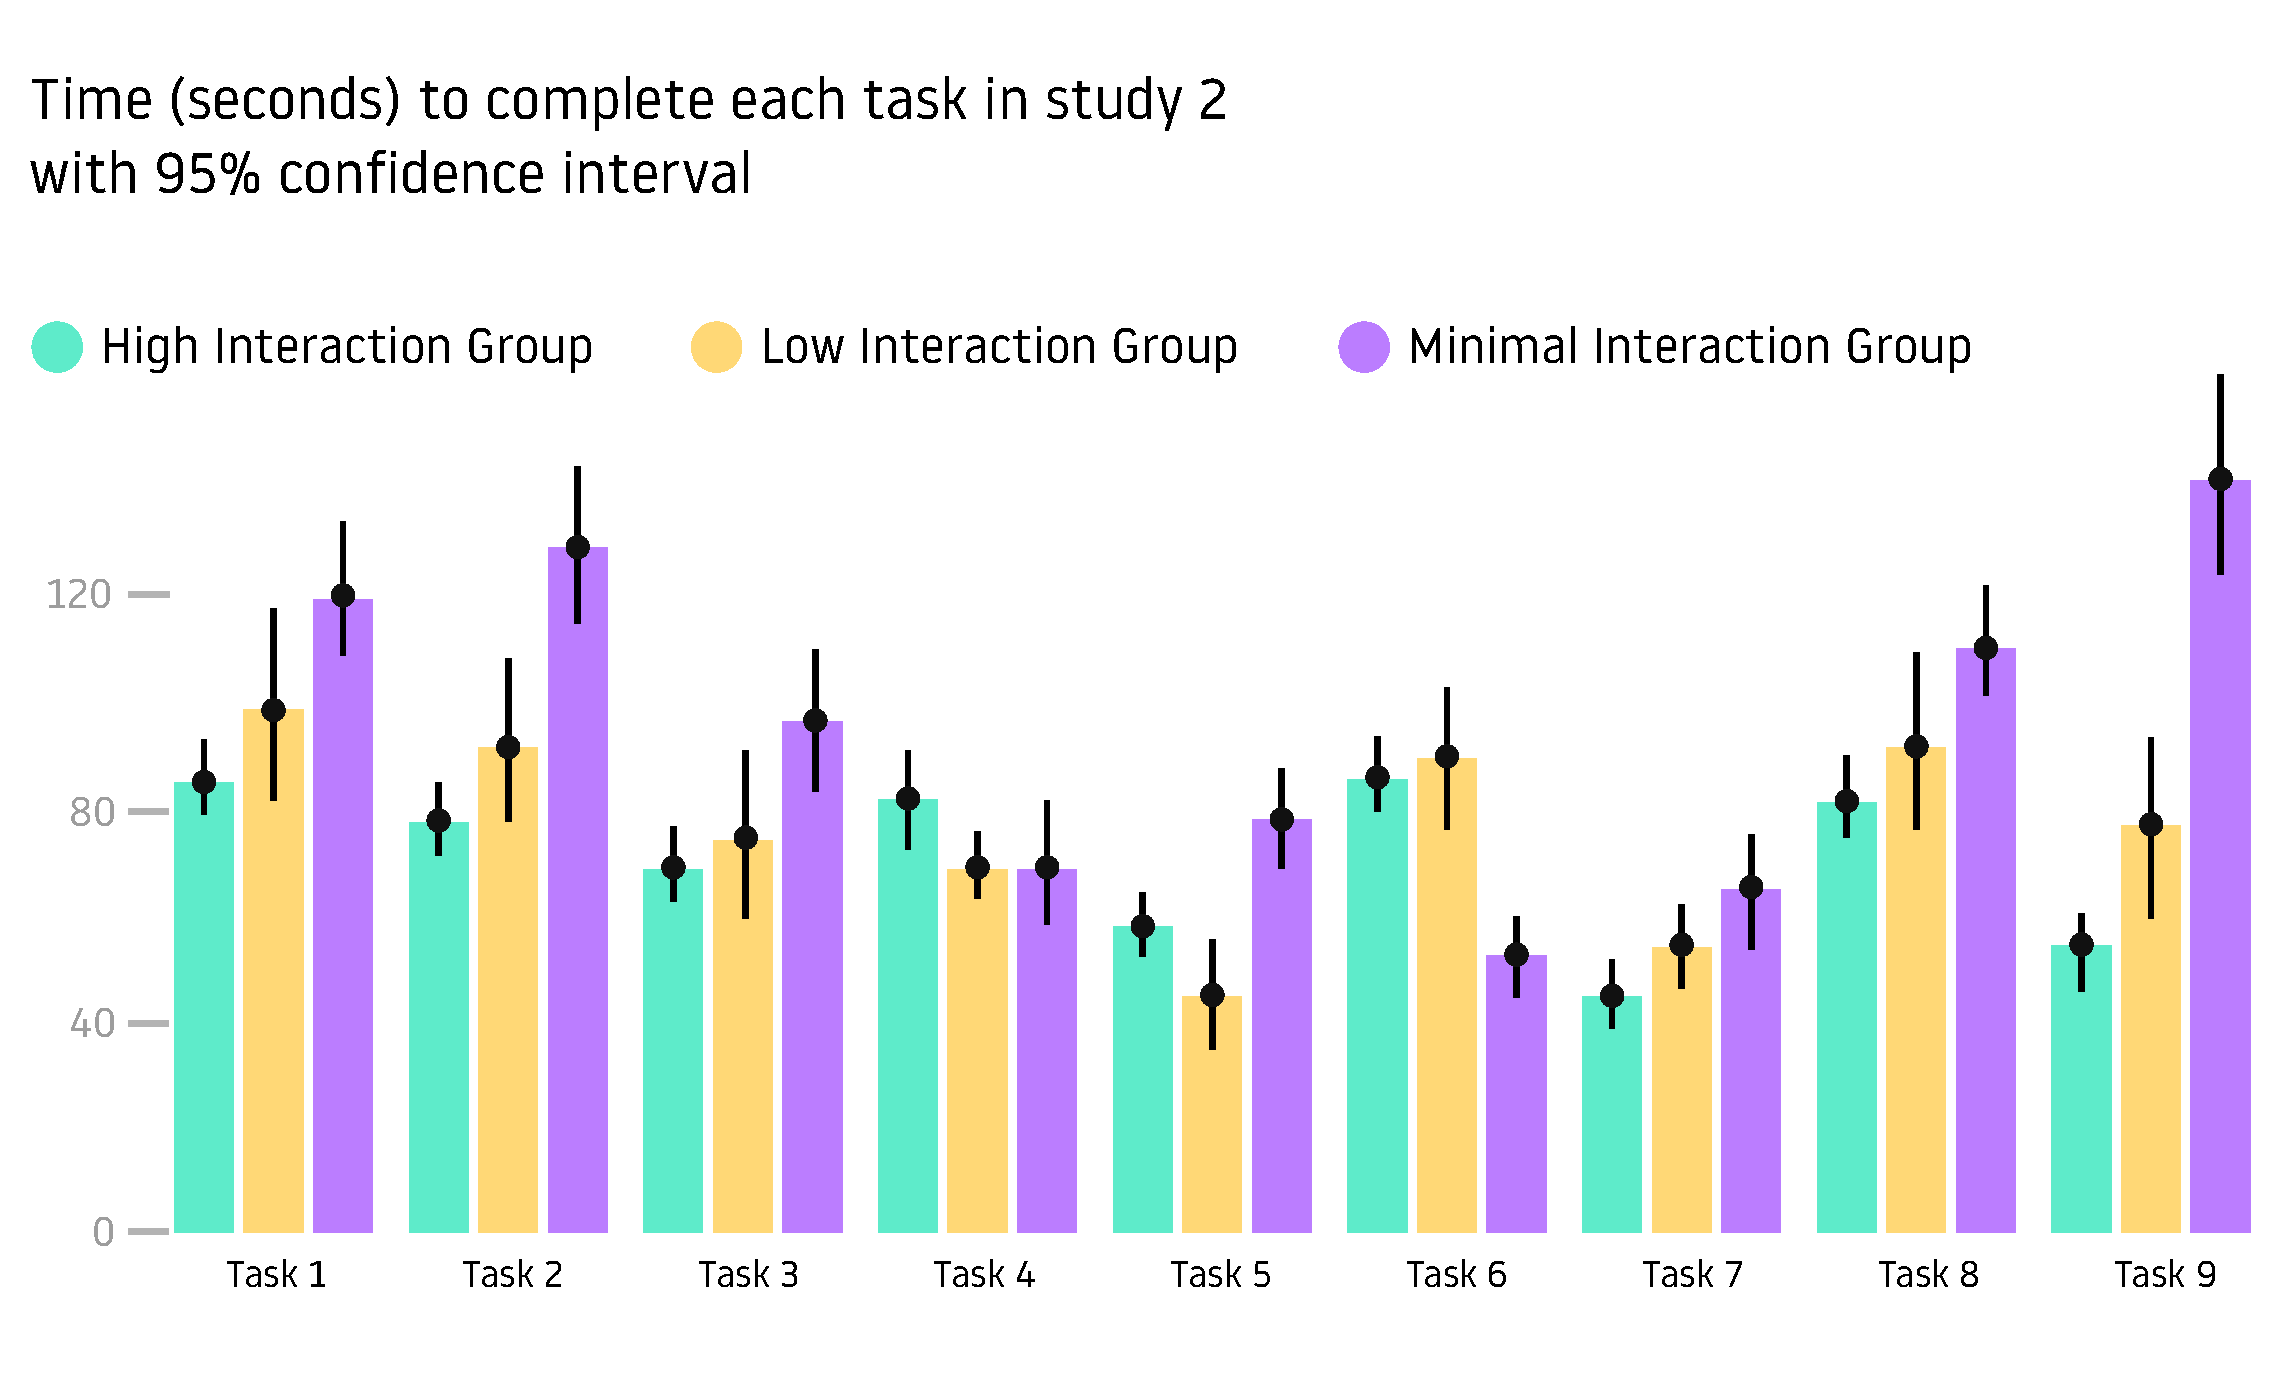
\includegraphics[width=\linewidth]{images/user-study-2.pdf}
    \caption{Time to complete by task in user study 2 with 95\% confidence interval}
    \label{fig:r4-analysis}
\end{figure}


% \begin{figure}[h]
%     \centering
%     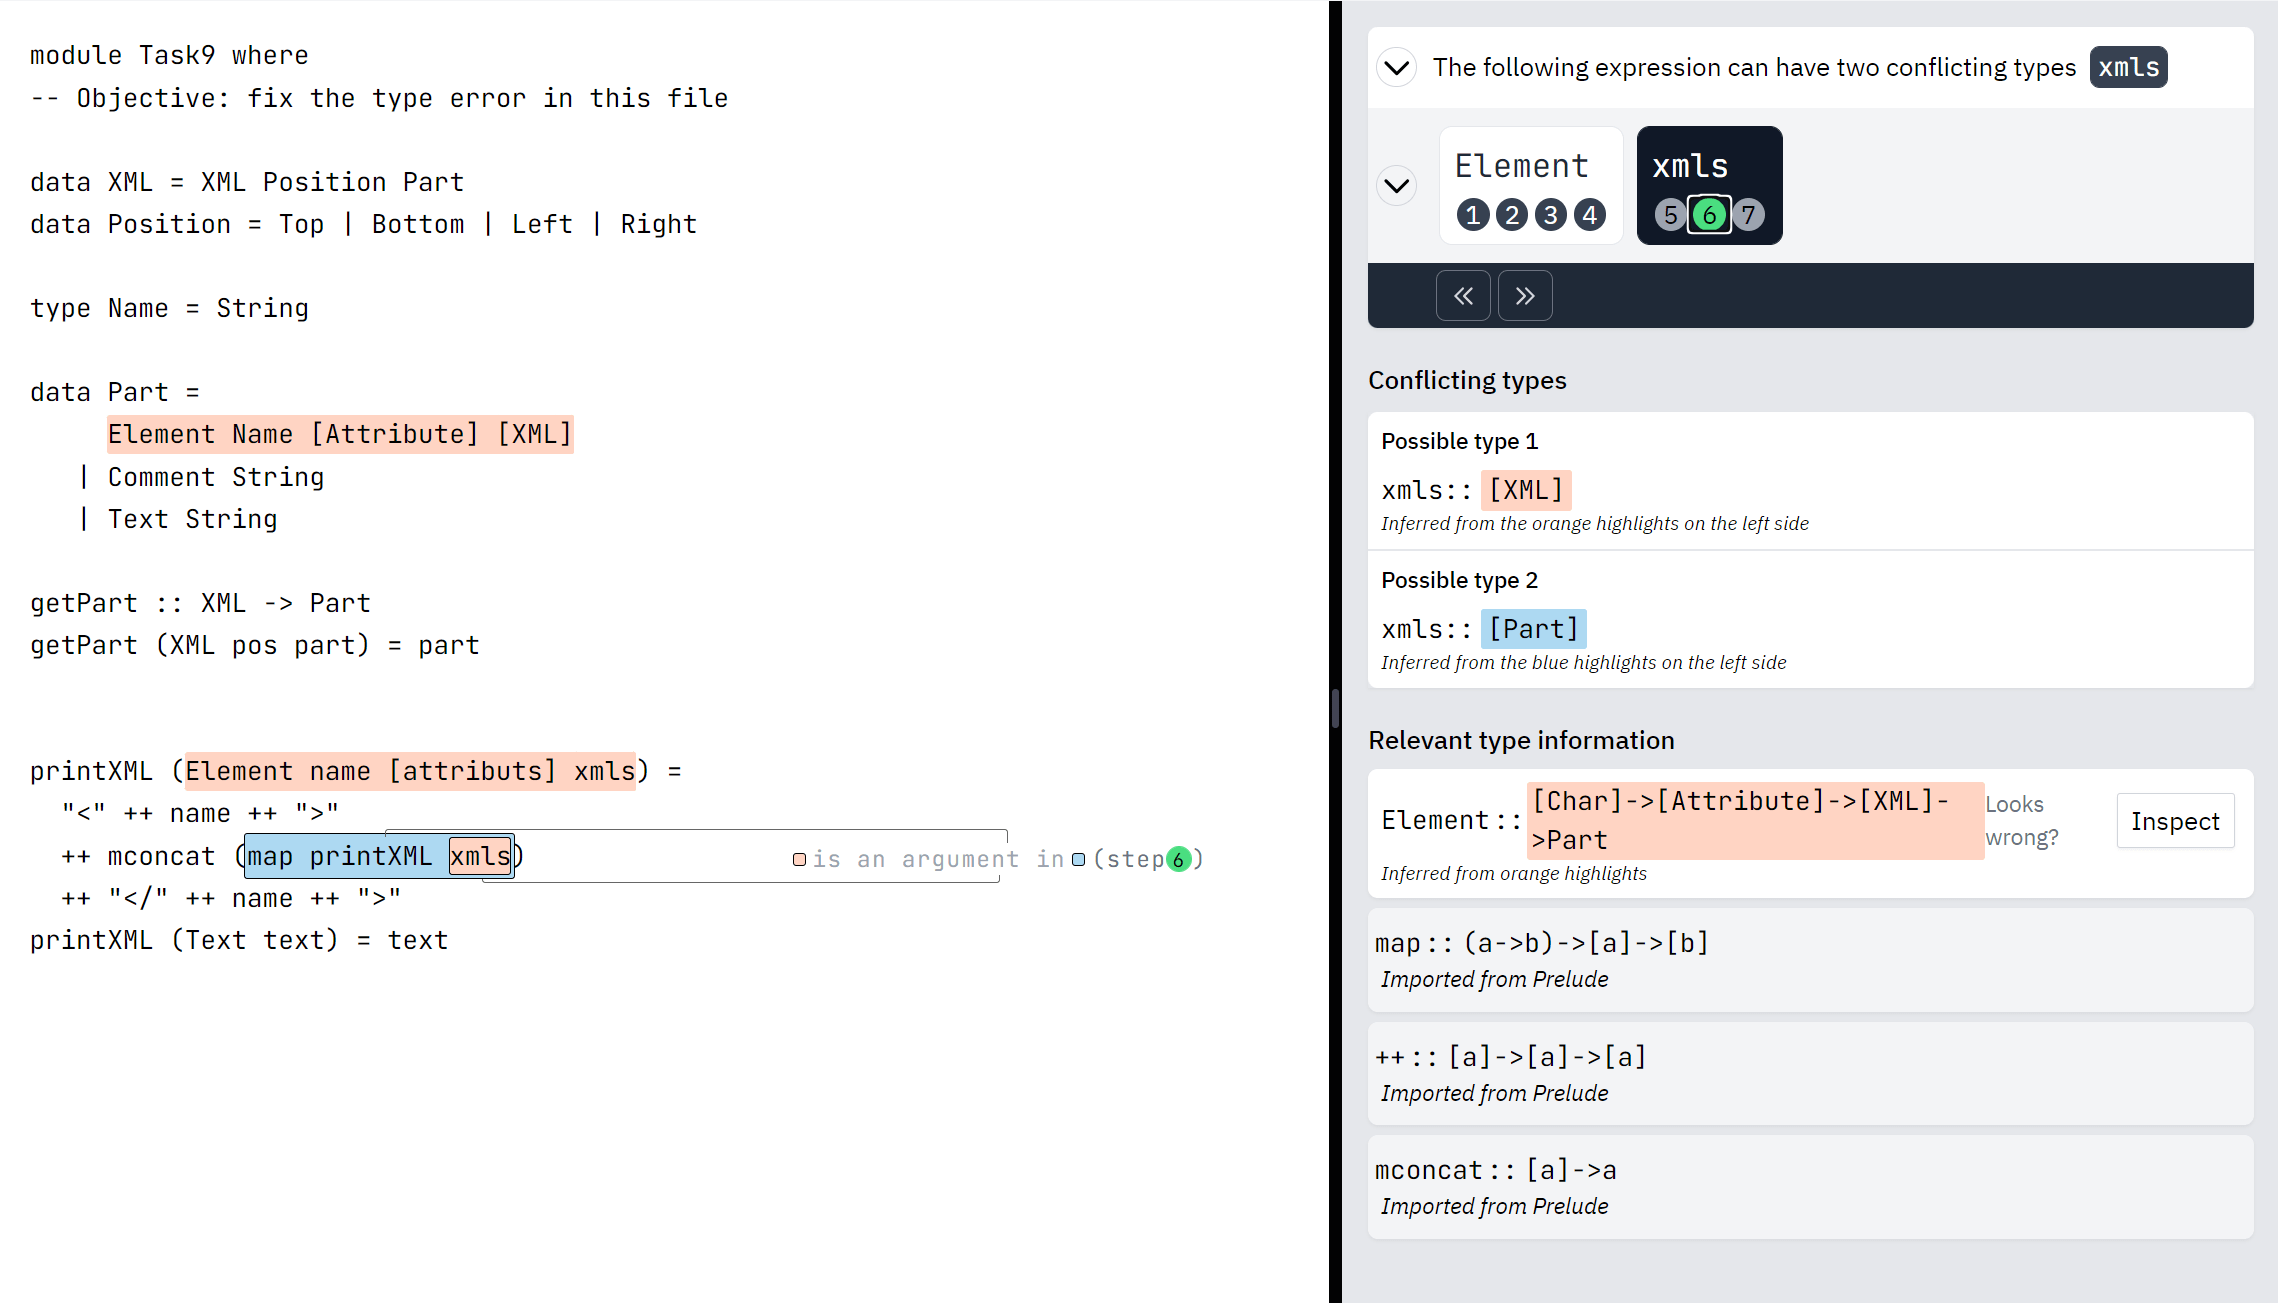
\includegraphics[width=\linewidth]{images/r4-task9.png}
%     \caption{
% High interaction users were able to locate the exact line for a potential fix after navigating to deduction step 6 or 7, which directly revealed the true cause of the type error. After this, 12 out of 15 high interaction users provided the most ideal fix in the first try. Low interaction group  takes longer time to examine the problem, provided wrong fixes in the initial trials. One participant fixed a minor run-time issue (a problematic pattern matching of `[attributes]` on line 18) however failed to identify the culprit of the type error.
%     }
%     \label{fig:r4-task9}
% \end{figure}


Another observation is when using the mode switching feature of \chameleon{}, programmers generally switching form a less informative display to a more informative one (Fig. \ref{fig:r4-mode-switching}). 

\begin{figure}[h]
    \centering
    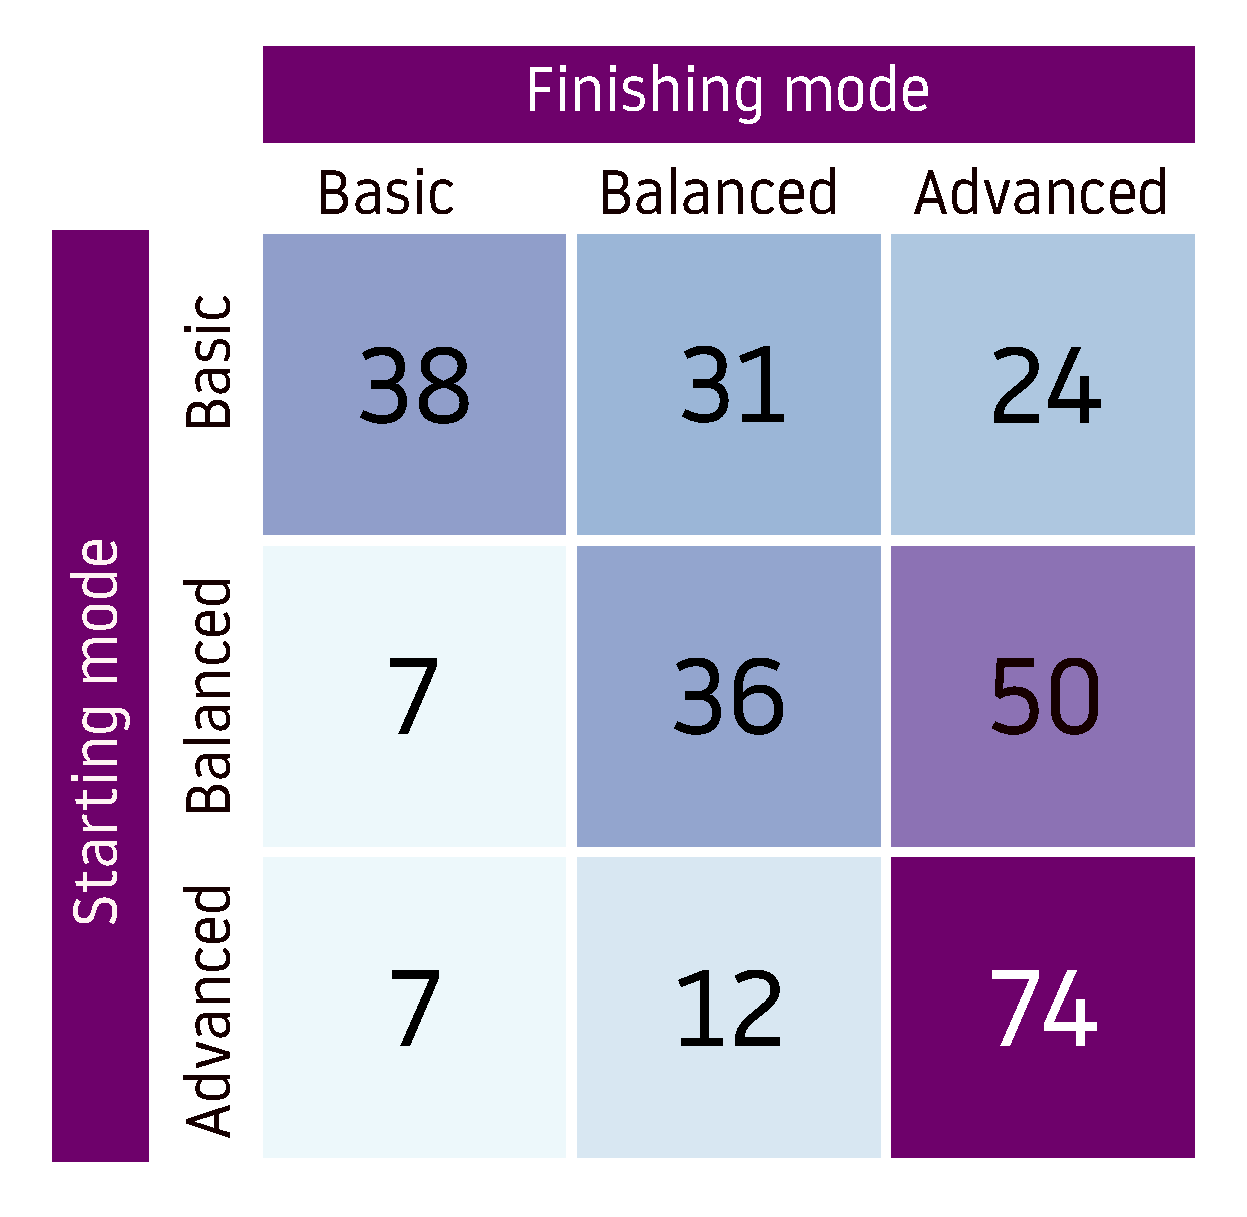
\includegraphics[width=\linewidth]{images/mode-switching.pdf}
    \caption{
        The rows represent the finishing mode, columns starting modes.
    }
    \label{fig:r4-mode-switching}
\end{figure}


